\documentclass{chi2009}
\usepackage{times}
\usepackage{url}
\usepackage{graphics}
\usepackage{color}
\usepackage[pdftex]{hyperref}
\hypersetup{%
pdftitle={kuczynski_rodriguez_scale_learning_produce_music},
pdfauthor={James Kuczynski, Joshua Rodriguez},
pdfkeywords={Q-Learning},
bookmarksnumbered,
pdfstartview={FitH},
colorlinks,
citecolor=black,
filecolor=black,
linkcolor=black,
urlcolor=black,
breaklinks=true,
}
\newcommand{\comment}[1]{}
\definecolor{Orange}{rgb}{1,0.5,0}
\newcommand{\todo}[1]{\textsf{\textbf{\textcolor{Orange}{[[#1]]}}}}

\pagenumbering{arabic}  % Arabic page numbers for submission.  Remove this line to eliminate page numbers for the camera ready copy

\begin{document}
% to make various LaTeX processors do the right thing with page size
\special{papersize=8.5in,11in}
\setlength{\paperheight}{11in}
\setlength{\paperwidth}{8.5in}
\setlength{\pdfpageheight}{\paperheight}
\setlength{\pdfpagewidth}{\paperwidth}

% use this command to override the default ACM copyright statement 
% (e.g. for preprints). Remove for camera ready copy.
\toappear{}

\title{Heptatonic Scale Learning To Produce Original Music}
%\subtitle{Heptatonic Scale Learning}
\numberofauthors{2}
\author{
  \alignauthor James T. Kuczynski\\
    \affaddr{Department of Computer Science}\\
    \affaddr{University of Massachusetts Lowell}\\
    \email{jkuczyns@cs.uml.edu}
  \alignauthor Joshua J. Rodriguez\\
    \affaddr{Department of Computer Science}\\
    \affaddr{University of Massachusetts Lowell}\\
    \email{jrodrig1@cs.uml.edu}
}

\maketitle

\begin{abstract}
In this paper we describe a heptatonic scale-based method of training an agent using Q-Learning and Markov decision processes to compose original music based on the tenements of Music Theory.  This novel approach allows our system to be entirely unbiased by the stylistic preferences of human composers.  We will also present an analysis of our results and discuss pros and cons of the method we employed against other existing methods.

\end{abstract}

\keywords{Q-Learning, Markov Decision Processes, Artificial Intelligence, Fourier Transform, Music Theory} 



\section{Introduction}

The idea of creating artificial intelligence to compose music is one which has sparked the imaginations of scientists for many decades.  As a discipline which is categorized as an art, it may seem impossible for an entity devoid of imagination and creativity to achieve such a goal.  However, music theory is a set of explicit rules which musical compositions follow.  These rules can be expressed as series of mathematical equations and logical expressions, making it possible for computer algorithms to interpret them.

However, most recent researchers in this field use pre-existing musical compositions created by human composers as input to train their AI.  This results in AI which are style-bound to a specific composer or set of composers.  Such an AI, if trained on Mozart's piano sonatas, will compose piano sonatas reminiscent of Mozart's style.  A recent approach was the use of an evolutionary algorithm on a Chomsky grammar-based representation of the music [2]. This grammar was composed of features such as
note, accidental (i.e. flat/sharp), note duration, etc. [ibid]. As input, the algorithm would receive themes composed by a human composer [ibid]. This method was reported to be successful at mimicking the style of a given composer; however, no quantitative results were published, probably as a result of the subjectiveness of music [ibid].  A similar method was implemented by Wiggins \textit{et al.} [3]. However, rather than create original compositions, it was used to develop variations of existing music works [ibid].

One of the challenges faced in this endeavor is training the AI [4]. Not only must it have built-in knowledge of music theory, but must be able to actively learn , in order to obtain for itself a unique and distinct personality [ibid]. The approach used by Hiller \textit{et al.} fails in this respect because a random number generator will always select random notes; it will not prefer certain equally-valid tones or progressions over others [1]. The method used by de la Puente \textit{et al.} does not have this shortcoming, but its preferences and biases which the AI will have are influenced by the melodies it listens to [2]. Also, Wiggins \textit{et al.} merely creates variations of a preexisting piece, rather than gaining a distinct personality [3]. Our algorithm focuses on the aspect of training an AI to learn to compose music in a given key by using Q-Learning to learn a heptatonic scale.  This learning method allows it to discover with rewards and penalties if a note is in a given key, or if not, then by how significantly it diverges.  It can then use this knowledge to create original compositions based on the fundamentals of music theory rather then the characteristics of a pre-existing composer.

An additional reason why training on heptatonic scales is a desirable characteristic is for potential future use as an assistive tool for teaching children--or adults--how to compose music. In Simon Holland's \textit{Computers and Music Education}, the author argues that artificial intelligence should be used in grade school to teach children the art of music composition [5].  Holland describes several existing systems which use built-in knowledge of music theory to assist the user [ibid].  Our system could easily be re-purposed for this task with very little modifications to the internal functionality required.



\section{Project Description}

This project is composed of a series of stages, which can be viewed as a series of interconnected modules.

\begin{figure}[htp]
\centering
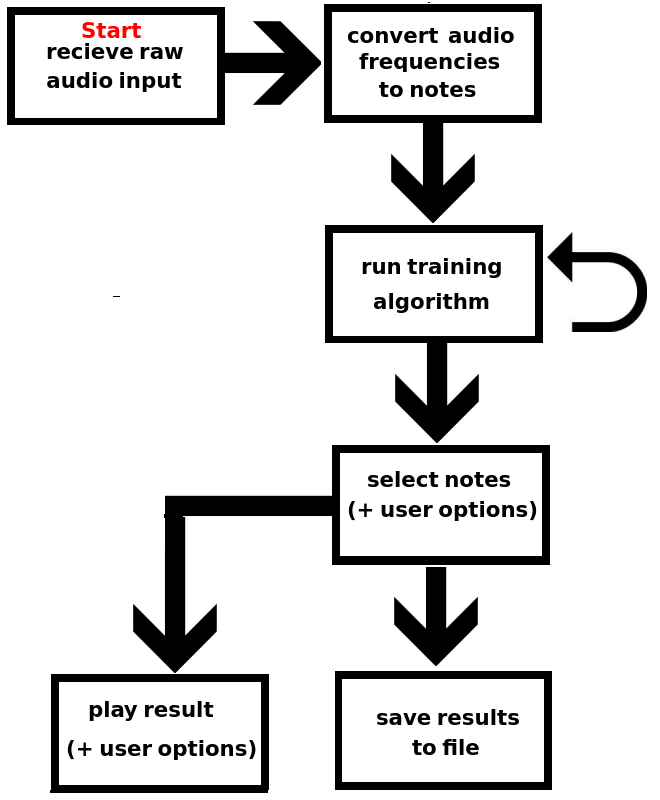
\includegraphics[width=5cm]{tmp}
\caption{System control flow}
\label{fig:controlflow}
\end{figure}


\subsection{Input Methods}

The method used to give the agent the goal scale was by playing live audio.  The user can play notes via an instrument (either acoustic or electronic), for our agent to listen to and receive.  The AI uses a fast Fourier transform (FFT) algorithm to compute the discrete Fourier transform (DFT).  The DFT is defined as follows:

let \textit{x}$_o$, ..., \textit{x}$_{N-1}$ be complex numbers.  Then
$$X_k = \sum_{n=0}^{N-1} x_ne^{-i2\pi kn/N} \hspace{1cm} \textit{k} = 0,...,\textit{N} - 1. $$

\begin{figure}[htp]
\centering
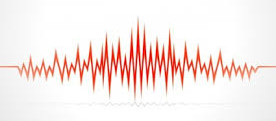
\includegraphics[width=8cm]{audio_wave}
\caption{Raw audio frequencies}
\label{fig:audio wave}
\end{figure}



This is an optimized version of the original Fourier Transform, which reduces the complexity from \textit{O}(\textit{n}$^2$) to \textit{O}(\textit{n} log \textit{n}).  This enables it to detect what notes are being played by parsing the dominant frequency.  Due to limitations in our sound recording device, the user was required to play each note multiple times for the AI to be confident that it has received the intended note.  Figure 3 demonstrates a series of notes being heard.  As can be seen, one particular note occurs the most frequently (red), and so it is assumed that the user is entering this particular note.  This allows the algorithm to work properly even when there is background noise.  The main logic for pitch detection was found in Ferdinand E. Silva's guitar tuner application using the PyAudio library.  We modified it mainly by including a confidence threshold.

\begin{figure}[htp]
\centering
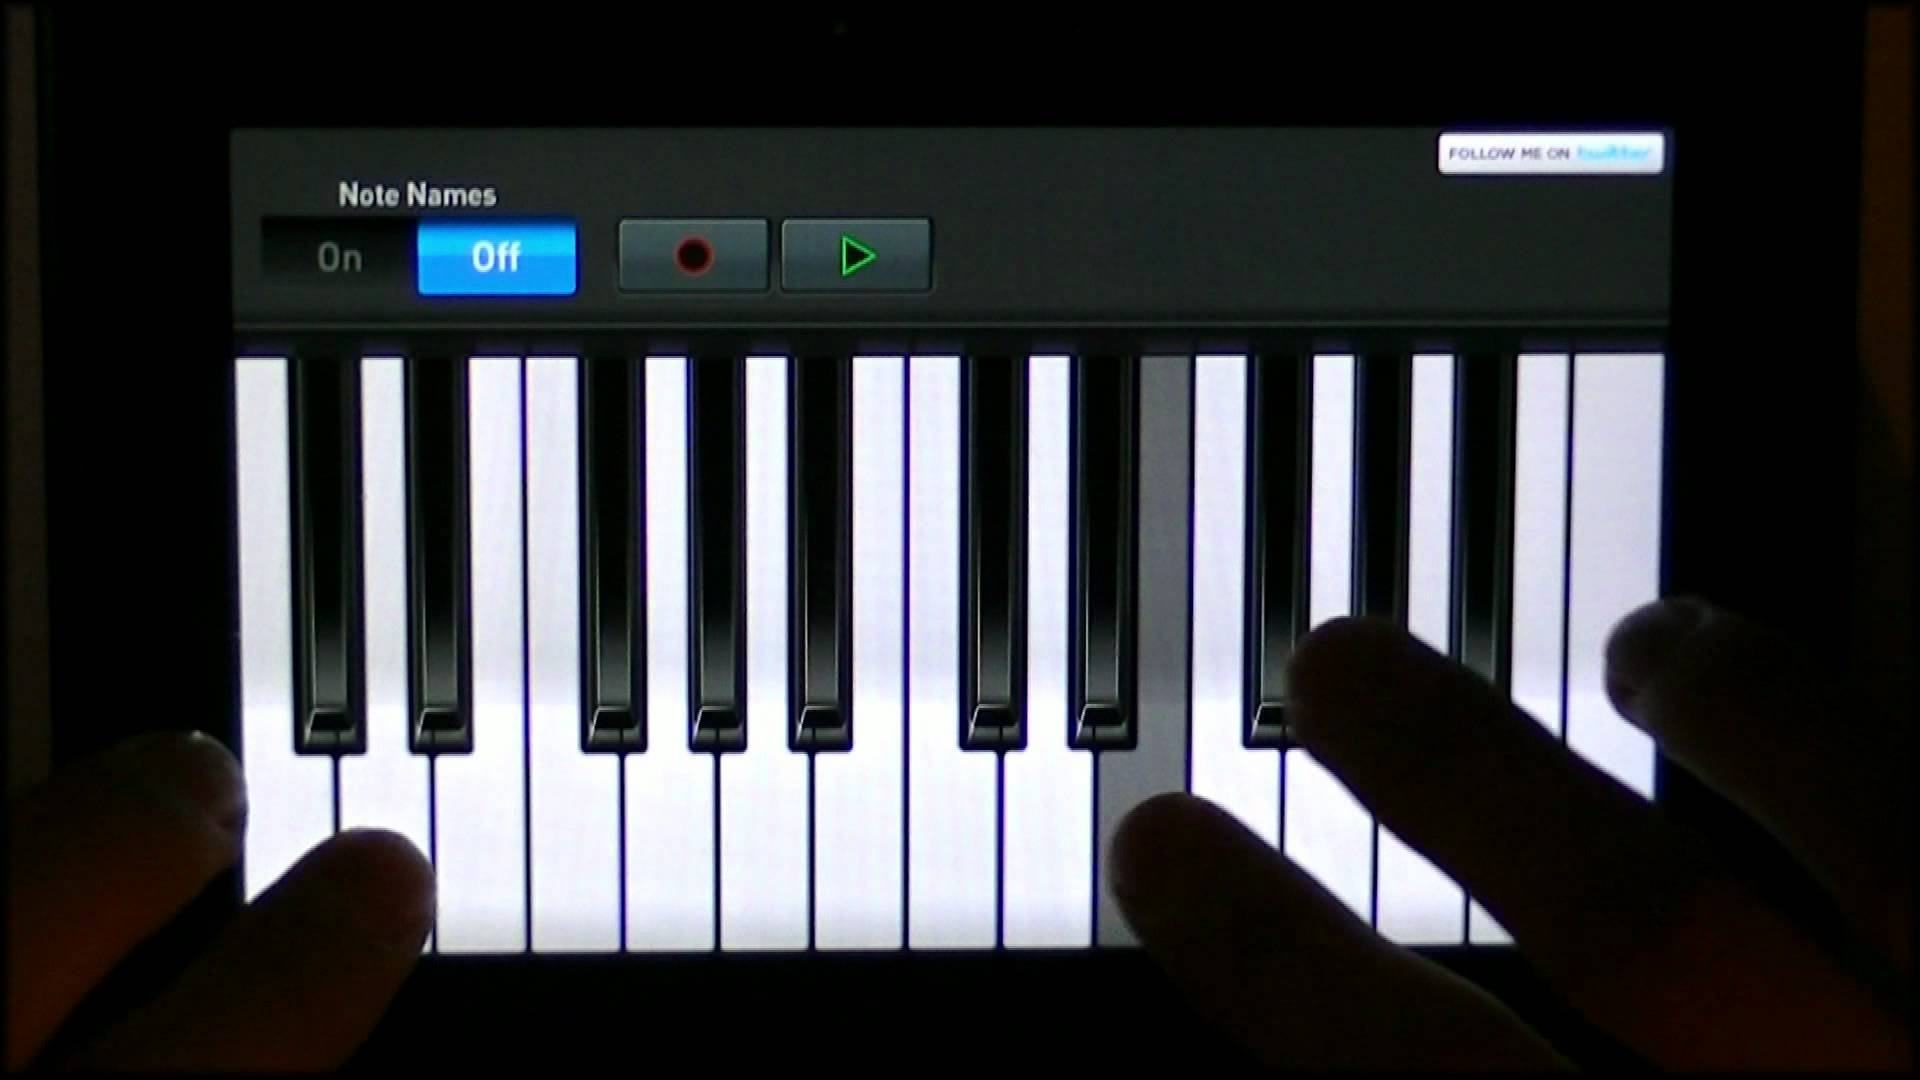
\includegraphics[width=8cm]{piano_app}
\caption{Tablet keyboard application}
\label{fig:piano_app}
\end{figure}

\begin{figure}[htp]
\centering
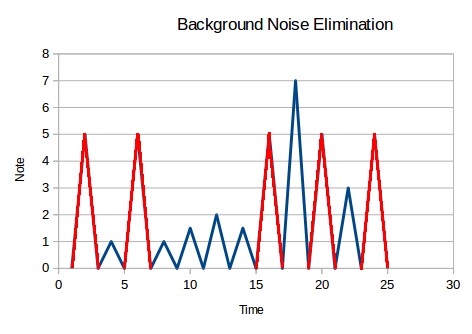
\includegraphics[width=8cm]{note_detection}
\caption{Input decoded}
\label{fig:frequencies}
\end{figure}

\begin{figure}[htp]
\centering
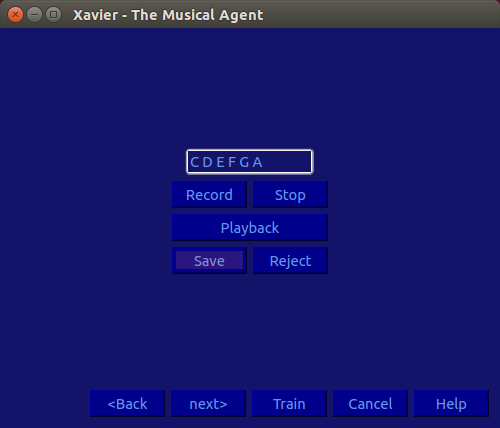
\includegraphics[width=8cm]{input_ui}
\caption{Audio input UI}
\label{fig:input_ui}
\end{figure}

The secondary method of input employed is passing the program a text-based representation of the notes as an array.  This was used during the implementation process since it was faster then receiving audio input from the user.  However, given how successful our aforementioned primary input method works, this mode was relegated for debugging use.

\subsection{World Representation}
The environment is fully observable, single-agent, deterministic, sequential, static, and discrete. It is fully observable because the agent has access to all notes that could ever be played in a scale. It is single-agent because there are no other agents working against or with it. It is deterministic because each action yields the desired consequence of playing that note. It is sequential because it learns what notes not to play through previous iterations. It is a discrete world of notes, which is fundamentally continuous due to the nature of frequencies.
\paragraph{States of The World}
The states of the agent's internal world has two components... \textbf{1) The last note played} 
\\
and 
\\
\textbf{2) How many notes have previously been played} 

Knowing the last note played is crucial for determining what note to play next.

Knowing how many notes have previously been played allows us to keep a First Order Markov Decision Process while not being entirely memory-less. If we did not include this component in our state we would need a Seventh Order MDP to solve a heptatonic scale.

There are two additive special states, namely the start and terminal states, which do not include a note component.


The entire state space is defined by...\\
\textit{(The total number of notes) $\times$ (how many previous notes could have been played [0 - 14]) + (The start and finish states) = $(12 \times 15)$ + 2 = \textbf{182 total states.}}

\paragraph{Transitions}
There are three sets of actions depending on a state. All actions are deterministic.


The start state can transition to any other state except the terminal state. There are 180 actions -- \\
\textbf{ACTION[\textit{StartState}]} = \textit{$\{$go to state $\|$ state $\in$ $\{$A, A\#, B, C, C\#, D, D\#, E, F, F\#, G, G\#$\}$ $\times$ $\{$0, 1, 2, 3, 4, 5, 6, 7, 8, 9, 10, 11, 12, 13, 14$\} \}$}


An ending state is defined as having fourteen notes previously played (a complete crescendo and decrescendo) or any note not in the original scale received. They have one action to finish and transition to the terminal state -- \\ 
\textbf{ACTION[\textit{EndingState}]} = \textit{$\{$go to TerminalState$\}$}


An intermediate state is defined as not being a start state or ending state. It can transition to any other state except itself, the terminal state or the start state. There are 179 actions -- \\ 
\textbf{ACTION[\textit{IntermediateState}]} = \textit{$\{$go to state $\|$ state $\in$ $\{$A, A\#, B, C, C\#, D, D\#, E, F, F\#, G, G\#$\}$ $\times$ $\{$0, 1, 2, 3, 4, 5, 6, 7, 8, 9, 10, 11, 12, 13, 14$\} - $\{$IntermediateState$\}$\}$}



\paragraph{Evaluation}
A collection of six reward cases guides our agent to learning the correct scale. It collects a large reward for being in an ending state with fourteen previous notes played and finishing. It collects a minor penalty for finishing on an ending state without fifteen previous notes played. It collects a large penalty for playing a note in the goal scale, but transitioning to a state with the wrong number of previous notes played. It receives a massive penalty for just playing out of sequence. It receives a minor penalty for transitioning to a state with a note not in the goal scale. It receives a reward for playing a note in the goal scale with the proper sequence.

\subsection{Learning Algorithm}
Our agent employs Q-learning as its AI backbone. The discount factor is a constant value of 1.0 because we want the agent to have a large horizon and prefer future rewards. This is beneficial due to the many rewards it accumulates in each time step. The learning rate is a constant 0.5 which is customary in learning rates for First Order MDP Q-learning. Each iteration of Q-learning puts the agent in the start state and each time step the agent transitions to a state and plays that note. If it transitions to the terminal state then that iteration of Q-learning ends.

\subsection{Exploration}
Our agent has the ability to explore off of the original goal scale to produce original music. This is done by taking the internal q-value map and taking the absolute value of all values greater than or equal to -750. The way our reward system works ensures all penalties up to -750 from a transition will still yield a note in scale. The agent can then choose to take an action from the modified q-value map as much as the user specifies on the exploration slider. The higher the slider the more the agent will choose his actions based on the modified q-value map. Every time the agent chooses an action from the modified q-value map it resets that value for that action to -1. This ensures it will encounter other q-values and not enter an endless loop.

\begin{figure}[htp]
\centering
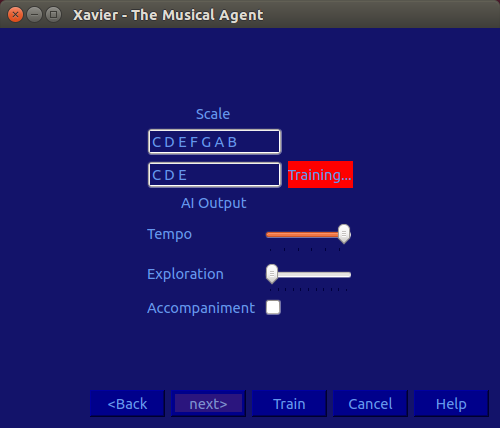
\includegraphics[width=8cm]{training_ui}
\caption{Training UI}
\label{fig:training_ui}
\end{figure}


\subsection{Output}

To facilitate a more accurate and verbose analysis of our work, this system supports several methods of output which run concurrently.  These consist of audio output which runs during runtime, and a text-based output which can be saved for reference and analysis.

\paragraph{Audio}

As the AI composes music, it plays it using MIDI output. The algorithm uses the PyGame library's MIDI module to produce the audio.  PyGame requires compatible audio drivers to be installed.  As we were running the system on an Ubuntu Linux operating system, ours used the default ALSA driver, which had to be manually started before running the application.  Our algorithm supports grand piano, church organ, and viola.  After selecting a note for the first voice to play, the AI then selects notes for the second voice (i.e. player).

\begin{figure}[htp]
\centering
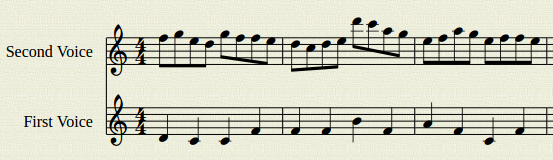
\includegraphics[width=8cm]{two_voices}
\caption{First and second voice}
\label{fig:two_voices}
\end{figure}


It does this by cross-referencing built-in rules of music theory against its current note to check which notes are compatible for the second voice to play.  The first voice always plays quarter notes, while the second voice plays eighth notes.  Thus, the ratio of notes played by the first voice to those played by the second voice is 1:2. The first note played by the later voice will be either a 3rd or a 5th above above the former voices note, and the second note will be either one note higher or lower.  For example, if the AI is in C Major and chooses the note C$_4$ as the primary note for the first voice, it will then randomly select one of the following tuples for the second voice:
$$\{(E_4, D_4), (E_4, F_4), (G_4, F_4), (G_4, A_4)\}$$



The second voice is also raised one octave above the first voice, and is given a lower volume, to help the audience differentiate between the two of them.



\paragraph{Music Score}

In order to have a permanent copy of results for analysis, we developed a method to convert 
the notes the AI selected into a musical score, also known as sheet music. In order to do this, we developed an algorithm to convert the \textit{(note, prevNumOfNotesPlayed)} tuples our AI used into LilyPond syntax, which is an audio programming language for notating music using ASCII characters, similar to LaTeX. 
LilyPond provides a compiler compatible with UNIX/Linux, Windows, and MacOS X systems which translates music from their custom LilyPond syntax text files into sheet music PDF documents.

\begin{figure}[htp]
\centering
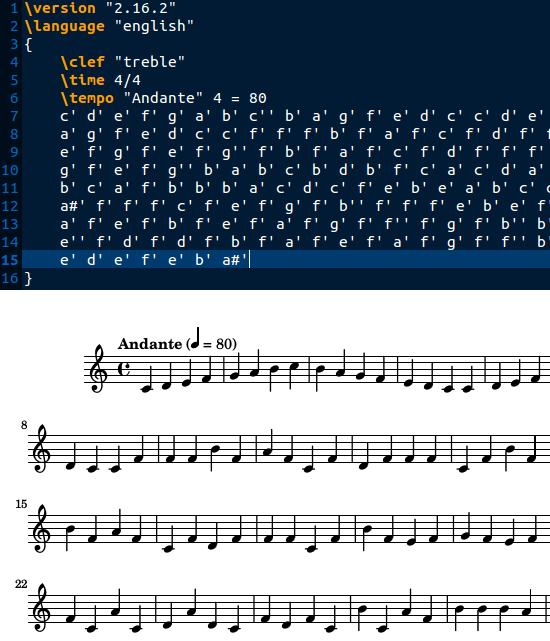
\includegraphics[width=8cm]{music_score}
\caption{Top: LilyPond music notation.  Bottom: LilyPond compiled music.}
\label{fig:lilypond}
\end{figure}

\section{Analysis of Results}

\begin{figure}[htp]
\centering
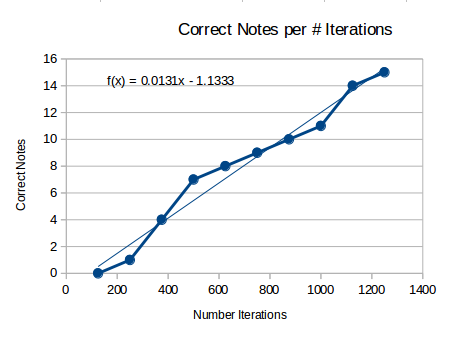
\includegraphics[width=8cm]{graph3}
\caption{Training Iterations}
\label{fig:training iterations}
\end{figure}

In order to test the robustness of our input method (i.e. our AI's ability to identify notes, even with background noise), we ran in during the class demonstration.  Despite the extremely loud environment, our algorithm successfully identified the correct notes being played by the user.

To test how many training sessions our algorithm required to successfully learn a scale, we ran it in increments of 125 iterations from [125-1250], measuring how many correct notes were played \textit{in the correct sequence}.  For example, in order to learn the C minor scale, it would have to correctly learn the following notes in sequence:
$$\{C_4, D_4, E^b_4, F_4, G_4, A^b_4, B^b_4, C_5, B^b_4, A^b_4, G_4, F_4, E^b_4, D_4, C_4\}$$
Thus, each scale consists of 15 notes, as can be seen represented in the y-axis of Figure 9.  The x-axis represents the number of iterations completed.  As can be seen in Figure 3, our AI always successfully learned the entire scale after training for 1250 iterations.  This confirms that our algorithm runs correctly.  We ran this analysis over 5 unique scales 5 times each, and our algorithm successfully learning the scale 100\% of the time, provided it was allowed to run for 1250 or more iterations.


To ensure the exploration was running correctly, we ran a series of tests with the exploration at 0, 25, 75, and 100 percent, respectively.  At each of these intervals we ran the program 5 times and recorded the number of notes in the scale which occurred.  As can be seen from Figure 10, as our exploration parameter increased, our AI varied farther from the original scale (and thus began to create original compositions).  It should be noted that the rate of change is rather hap-hazard.  This is partially because of the large variance in results between runs.

\begin{figure}[htp]
\centering
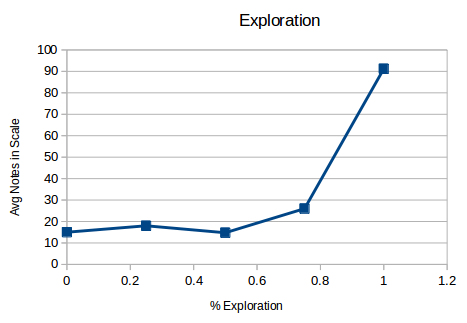
\includegraphics[width=8cm]{graph2}
\caption{Exploration}
\label{fig:exploration}
\end{figure}
\section{Discussion}

While many of the skills used on this project were ones which we learned in class with Dr. Fred Martin, still others were ones which we studied on our own to enhance the performance of our system.

At Dr. Martin's recommendation, we investigated higher order Markov decision processes. We determined we could have implemented our system this way, but by including a memory component into our state representation, we did not need a higher order MDP.

One thing we learned was genetic mutation algorithms, which are methods which have been used in similar projects in the past.  In the end we opted not to use these on account of their dependence to pre-existing human-composed music, and also because we wanted to try a method which was never used before to the best of our knowledge.

One of the most frustrating challenges we encountered while developing this application was getting the PyGame MIDI output API to function correctly.  We discovered that manipulating audio device drivers which function as kernel daemons takes some skill.  Fortunately, we were able to come up with an un-invasive solution.  This was especially important because we wanted other people to be able to run our program without having to modifying system configuration files.

\paragraph{\textbf{Ethical Implications of This Work}}

As with many other applications of artificial intelligence, there are possible ethical implications of this work.  The advancement of AI capable of composing original music could lead to a severe degradation of the art of music which at its peak could generate all songs in the future as opposed to humans.  It may appear to many that such an event is very distant; however, it should be noted that this is still a potential eventuality.  Hardware and software continually improve--thus raising the performance of AI--and these optimizations are likely to continue to improve in the future.

However, it should be noted that artificial intelligence would only replace human composes in such a situation if the AI were \textit{fully autonomous}.  If, on the other hand, it was merely an \textit{assistive} AI, such as Hilbert [1] describes, then it could allow human composers to produce compositions faster and more efficiently, rather then taking over their jobs.  Is it possible that even an assistive AI could result in a negative ethical impact?  This may be possible, but at least the likely-hood is greatly mitigated.


\section{Conclusions}

We have presented a method of training an artificial intelligence to compose original music compositions using a heptatonic scale model.  Our system successfully learns scales using Q-Learning and uses its knowledge of music theory to create original scores.

One of the drawbacks to this method is that--although it achieves the goal of avoiding biases and preferences of existing human composers, in its current form it produces music which is utterly devoid of any kind of emotion or feeling.  Given the current climate and trends of popular music, many may perceive this as a negative characteristic.

There are several directions in which we plan to enhance our system in the future.  Our AI currently produces music for up to two instruments.  However, we intend to expand our system to write music for a larger number of voices or instruments, such as a string quartet.  Given that our AI identifies what notes are compatible with others in a given key, another possible use for this program would be as an assistive tool for teaching children, such as those proposed by Simon Holland [5].

With more time we would overhaul our system into a stochastic process. The probabilities would be reliant on which genre of music our agent is trying to play. We would have to analyze many musical pieces to find how likely it is for a note to played in that genre of music [4]. 
\section{Acknowledgments}

The work described in this paper was conducted as part of a Fall 2016 Artificial Intelligence course, taught in the Computer Science department of the University of Massachusetts Lowell by Prof. Fred Martin.  We would also like to thank Dr. Heidi Furey for raising our attention to the ethical concerns of artificial intelligence, and Dr. Carmen Rodriguez-Peralta (Ph.D. in Piano Performance) for her suggestions on how to accurately evaluate our output.  We would also like to thank Dalton Curtin for lending us audio devices, and Daniel Brooks for his advice regarding a proper collaborative software work-flow using Git.


\begin{thebibliography}{9}
\bibitem{one} 
McAlpine, Kenneth, Eduardo Miranda, and Stuart Hoggar.  1999.  "Making Music with Algorithms: A Case Study System." \textit{Computer Music Journal} 23, 2 (Summer):19-30.

\bibitem{three}
A.O. de la Puente, R.S. Alfonso, and M.A. Moreno.  "Automatic Composition of Music by Means of Grammatical Evolution".  In \textit{Proceedings of the 2002 conference on APL: Array Processing Languages: Lore, Problems, and Applications}, pages 148-155, 2002.

\bibitem{four}
Wiggins, Geraint, George Papadopoulos, Somnuk Phon-amnuaisuk and Android Tuson, in \textit{International Journal of Computing Anticipatory Systems}, 1998.

\bibitem{five}
Papadopoulos, George, and Geraint Wiggins, "AI Methods for Algorithmic Composition: A Survey, a Critical View and Future Prospects", in \textit{AISB Symposium on Musical Creativity}, 1999, pp. 110-117.

\bibitem{six}
Holland, Simon. "Artificial Intelligence, Education and Music: The Use of Artificial Intelligence To Encourage and Facilitate Music Composition by Novices," CITE Report No. 88, Centre for Information Technology in Education, 309 pages 1989.
 

\end{thebibliography}
\end{document}
